
So keeping in mind, the goal here is to reduce away the model-view-update-cycle. To demonstrate how this works, we do it by example, and in this section we describe a Jali implementation of the Elm-model (or model-view-update?), which we will later reduce. Take as example a website with a single counter on the screen, and two buttons; one that increments and one that decrements the counter. In an elm like application, state is stored in the model, an update function defines how to handle each possible action, and the structure of the view is defined in the view function. The corresponding Jali program can be found in figure \ref{JaliMeetsElm}. 

\lstinputlisting[label=JaliMeetsElm, language=Jali, caption=Button example in Jali]{./code/button.jali}

To store the state of the counter it has a simple model which is just an integer set to 0. 

It has two actions \texttt{Increment} and \texttt{Decrement}. The \texttt{update} function either increments or decrements the model, depending on the given action. 

A view is represented by the \gls{adt} \texttt{Node}, which can either be a \texttt{Tag}, representing \gls{html} elements like <div></div> or <p></p>, or a \texttt{Text} node, which represents the plain text that can be written within \gls{html} elements. A \texttt{Tag} takes three arguments; a string to denote the type of the tag (e.g. a 'div'), a list of attributes, and finally a list of nodes to denote its children (inner elements?). A \texttt{Text} node is a leaf node and can only contain text. To illustrate how this data type can be used to represent an \gls{html} page with a counter an to buttons, see the \texttt{view} function in the code listing \ref{JaliMeetsElm}. When given a model, in this case an integer, the  \texttt{view} function returns the view with the model inserted as the counter. So giving the view function the initial model 0 generates an ADT of value of 'Tag' corresponding to an \gls{html} page with two buttons and a counter set to 0.


\liv{should we show the generated adt?} % Running the Jali program through the interpreter will generate our initial view represented as an \gls{adt} value of 'Tag'.
% \lstinputlisting[language=Jali, caption=View output]{./code/button-output.fs}
\\
The \texttt{viewToHTML} function translates the \gls{adt} into \gls{html}, which can be displayed in the browser as seen in Figure \ref{fig:buttons_in_browser}. 
\liv{Jan: i need yo help here; should the workings of this be elaborated?\\
Søren: Should we display the translate function and the html ouput? In appendix or here?} %this happens in the ?? function, and the output can be found in Appendix ??. 

\begin{figure}
    \centering
    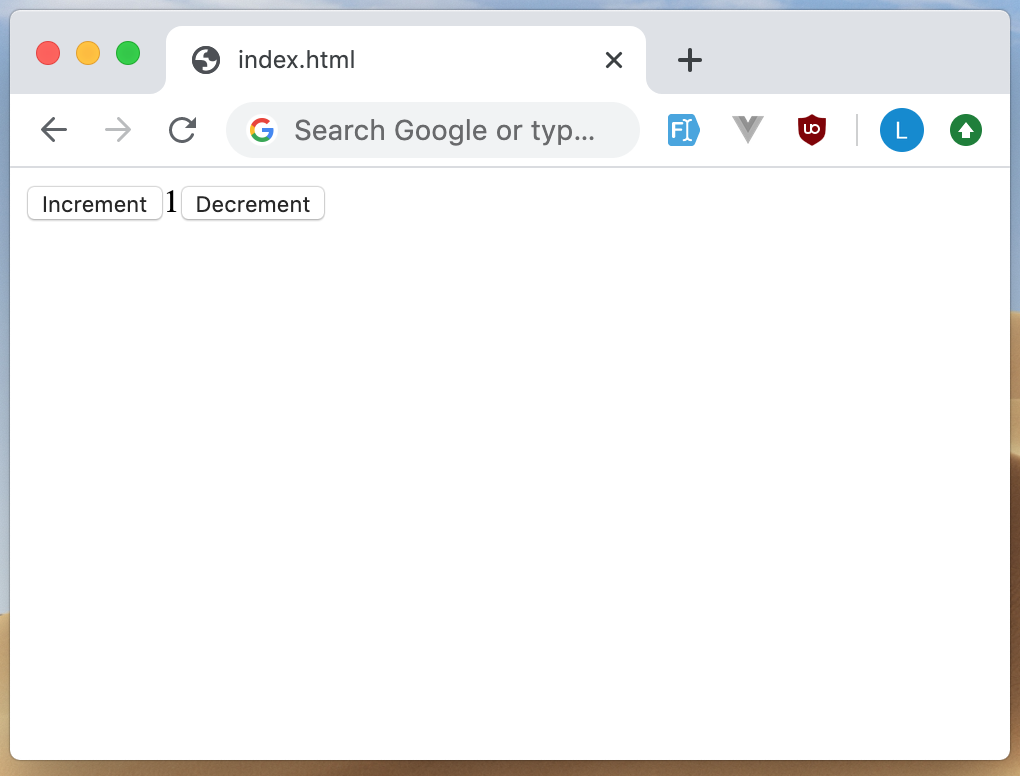
\includegraphics[width=\textwidth]{images/jali-button-in-browser.png}
    \caption{Jali button view displayed in browser}
    \label{fig:jali-buttons-in-browser}
\end{figure}


\liv{How to display the diff and patch function? }

However, pressing these buttons will not do anything without any JavaScript code. That is, from our model, we also need to generate the JavaScript that knows what should happen when we press the button. This is where partial evaluation will help us. 



% Running the Jali program through the interpreter will generate our initial view represented as an \gls{adt} value of 'Tag'.
% \lstinputlisting[language=Jali, caption=View output]{./code/button-output.fs}

The \texttt{viewToHTML} function translates the \gls{adt} into \gls{html}, which can be displayed in the browser as seen in Figure \ref{fig:buttons_in_browser}. 
\liv{Jan: should the workings of this be elaborated?\\
Søren: Should we display the translate function and the html ouput? In appendix or here?} %this happens in the ?? function, and the output can be found in Appendix ??. 

\begin{figure}
    \centering
    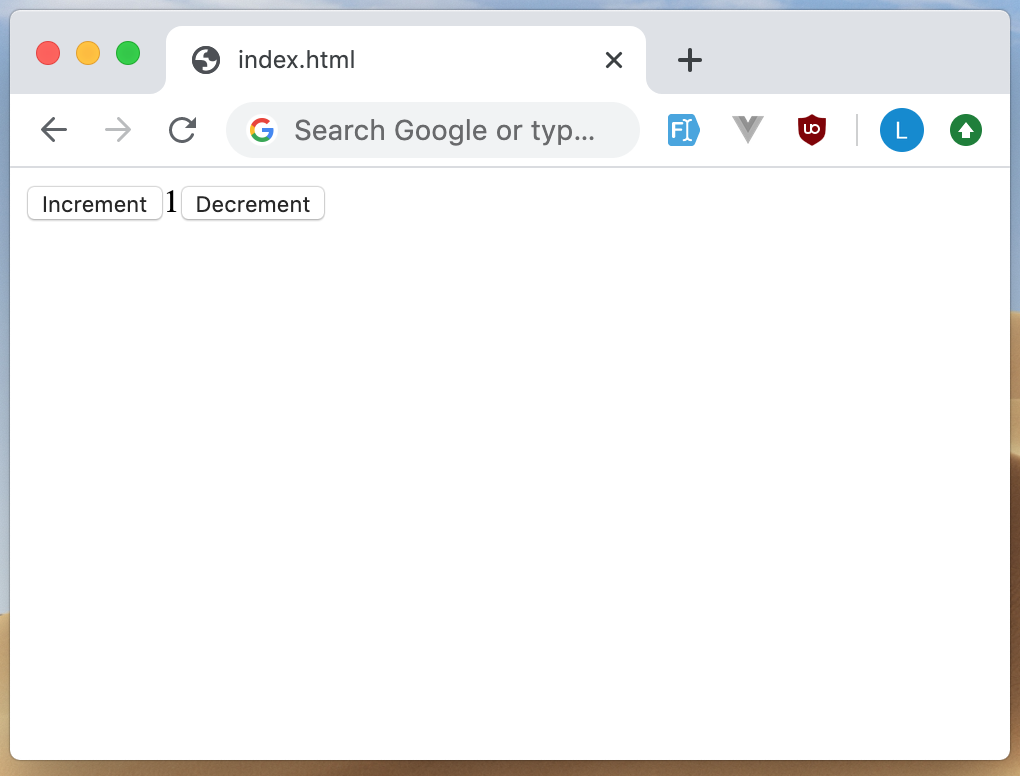
\includegraphics[width=\textwidth]{images/jali-button-in-browser.png}
    \caption{Jali button view displayed in browser}
    \label{fig:jali-buttons-in-browser}
\end{figure}

However, pressing these buttons will not do anything in plain html without any JavaScript code. 




We then have a diff function, which takes two views, and returns a data structure that describes the path to all differences between the two views.

\begin{verbatim}
    diff: View -> View -> DOM-Update-Actions
\end{verbatim}

Assume that we have a current view based on the current model m. When a user event triggers some action a on the model m, the functions are applied as follows:

\begin{verbatim}
    diff current_view (view (update a m))
\end{verbatim}

We update the model m with a, and then call view the get the view of the new model. Then we diff the old view with the new view, to get the changes that needs to be applied to the current view. 
\\\\
Now all we need is a patch function, which takes the initial view and the returned structure from the differ function and applies the changes onto the passed view, returning a new view with all fields updated.

\begin{verbatim}
    patch: View -> DOM-Update-Actions -> View
\end{verbatim}

%\lstinputlisting[label=JaliMeetsElm]{}



% \liv{should we just get rid of 'patch'?}
% \jan{no, as it is useful to show what the JaLi can do}
% The view function, takes a model and returns a string that represents the structure in form of valid \gls{html}. The update function takes an action and a model and updates the model accordingly. To demonstrate how this works, we construct a simple example consisting of two buttons: \textit{Increment} and \textit{Decrement} and a paragraph element displaying a counter, that can be altered by using the buttons respectively. The corresponding JaLi program can be found in figure \ref{JaliMeetsElm}. 

% \lstinputlisting[label=JaliMeetsElm, language=Jali, caption=Button example in JaLi]{./code/button.jali}

% To store the state of the counter it has a simple model which is just an integer set to 0. 

% The \texttt{view} function describes the view, in terms of the \gls{adt} \texttt{Node}. To illustrate how this data type can be used to represent an \gls{html} page with a counter an to buttons, see the \texttt{view} function in the code listing \ref{JaliMeetsElm}. A \texttt{Node}, can either be a \texttt{Tag}, representing \gls{html} elements like \texttt{<div></div>} or \texttt{<p></p>}, or a \texttt{Text} node, which represents the plain text that can be written within \gls{html} elements. A \texttt{Tag} takes three arguments: a string to denote the type of the tag (\textit{button}), a list of key-value pairs that are called attributes (\textit{value=42}), and a list of child nodes, which are the nested tags in this element. A \texttt{Text} node is a leaf node and can only contain text.
% In this example, the \texttt{view} function takes an integer as argument and returns the view with the model inserted as the counter: when the top button is pressed, \texttt{update Increment} is called, and when the lower button is pressed, \texttt{update Decrement} is called. 

% By giving the view function the initial model 0 we get an ADT of value of 'Tag' corresponding to an \gls{html} page with two buttons and a counter set to 0.

% \liv{ How to proceed? }
% \jan{explain the other functions and show example outputs}
% \liv{should we show the generated adt?} 
% \jan{yes}
% % we use the evaluater on the Differ (Diff (view init) (view (update Increment) init) -> and then translate that to javascript
% \jan{write about diffing and what happens and pretend JavaScript compiler exists, show outputs}
